datasheets ne555, 2n2222, octave
\paragraph{Introducci\'on}
En este apartado se expondr\'a el diseño del transmisor, los c\'alculos matem\'aticos necesarios, simulacion por ordenador y los resultados practicos.
El transmisor está diseñado para generar una modulación ASK y emitir a una frecuencia de $30Mhz$. La frecuencia de emisión se sintoniza con la del receptor por medio de un condensador de capacidad variable.
\paragraph{}
NO REPETIR, EXPLICAR LA FOTO
En la figura \ref{fig:tx} se puede observar el esquema eléctrico del transmisor.
El principio de funcionamiento del transmisor es un oscilador, basado en un par resonante LC, el cual fija la frecuencia de emisión. Esto se realiza realizando un bucle de realimentación positiva, donde el transistor NPN juega el papel de elemento activo de amplificación, el circuito tanque LC es el filtro que permite que en cada iteración del bucle, se amplifique la frecuencia deseada. mientras que el condensador de realimentación, genera la realimentación positiva, sumando una fracción de la salida con la señal de entrada, que en este caso es el propio ruido generado por el circuito.
El circuito se diseña para disipar la mayor potencia posible para que la señal alcance la mayor distancia posible. 
Por otra parte, el cicuito permite modular la señal portadora eléctricamente cortando y produciendo la oscilación en función de las variaciones de la señal moduladora. Esto es posible gracias al segundo transistor PNP, el cual trabaja en corte y saturaci\'on y corta el paso de corriente general del circuito.
% Esto se realiza por medio de un oscilador Colpitts en base común sintonizado a la frecuencia de emisión y que a su vez es mezclado con una señal de onda cuadrada generada por el chip integrado NE555.
% La señal de onda cuadrada generada por el NE555, es modulada en frecuencia, por dos pulsadores, produciendo dos diferentes canales digitales de salida.
El esquema completo del transmisor se expone en la figura \ref{fig:tx}.

\begin{figure}[h]
    \centering
    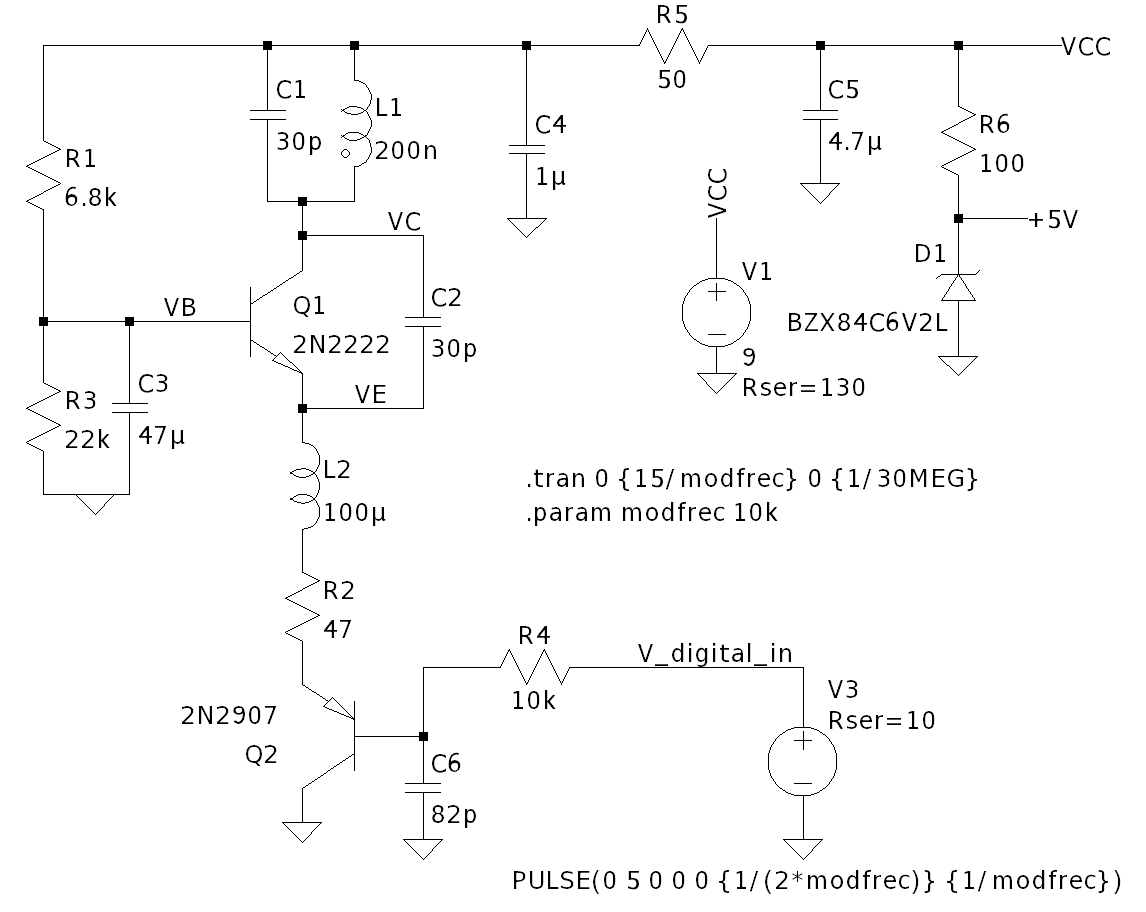
\includegraphics[scale=1, width=1\textwidth]{transmisor}
    \caption{Esquema el\'ectrico del transmisor}
    \label{fig:tx}
\end{figure}

\paragraph{Diseño del oscilador}
\paragraph{Polarizaci\'on:} IGUAL Y MENCIONANDO EL TRANSISTOR PNP EN CORTE APROX 0.2 V DESPRECIABLE.
En primer lugar se debe fijar el punto de operación deseado. Se deben tener encuenta dos cosas: la zona trabajo del transistor y la potencia del circuito. La zona de trabajo debe ser activa directa, pues para producir la oscilación, el bucle de realimentación positiva debe tener la etapa de amplificación proporcionada por el transistor. La potencia del circuito, junto a la fracuencia de diseño, acotan el modelo de transistor que se ajuste al circuito.
En primer lugar se necesita un transistor con una frecuencia de transición $f_t > \SI{30}{\mega\hertz}$. Aparte el parámetro $I_{Cmax}$ debe ser suficiente para proporcionar la potencia deseada sin deteriorarse. Se elige un transistor 2N2222, cuya $f_t > \SI{30}{\mega\hertz}$ e $I_{Cmax} = \SI{0.6}{\ampere}$ y una $V_{CC} = \SI{9}{\volt}$. Se fija $Ic = \SI{80}{\milli\ampere}$, que supondr\'a una potencia de aproximadamente $I_C \cdot V_{CC} = \SI{0.72}{\watt}$ y $V_{CE} = \frac{V_{CC}}{2} = \SI{4.5}{\volt}$ condici\'on necesaria para trabajar en activa directa. Además, de la hoja de características del 2N2222 se conoce $h_{FEmax} \approx 300$, aunque medido con un mult\'imetro, nos da el valor $h_{FE} = 280$ por lo que se utilizar\'a este \'ultimo.
En lugar de repetir el cálculo que se hizo para seleccionar el valor de las resistencias de polarización, se optará por comprobar si los valores elegidos satisfacen las imposiciones.
\paragraph{}
Se utiliza equivalente de Thevenin para las resistencias en paralelo. En la malla que aparece se obtiene:
$$V_{th} - 0.7 - I_c \cdot R_e = I_b \cdot R_{th}$$
Siendo:
\[
\begin{array}{rl} 
      \begin{array}{l}
	 V_{th} = \frac{V_{CC} \cdot R_2}{R_1+R_2} \\
	 R_{th} = \frac{R_1 \cdot R_2}{R_1+R_2}
      \end{array}
      &
      \begin{array}{l}
	 I_b \cdot h_{FE}= I_c \\
	 h_{FE} = 280
      \end{array}
\end{array}
\]
Se obtienen $I_c$ y $V_{CE}$ con las siguientes dos ecuaciones sustituyendo los valores correspondientes:
\begin{align*}
   R_1=\SI{10}{\kilo\ohm} \quad R_2=\SI{20}{\kilo\ohm} \quad &R_E=\SI{40}{\ohm} \quad V_{CC} = \SI{9}{\volt} \\
   I_c \cdot \left( 40+ \frac{R_{th}}{h_{FE}}\right) &= V_{th} - 0.7 \\
   V_{CC} = V_{CE} &+ I_C \cdot R_E \\
   V_{CE}= \SI{5.68}{\volt} \quad& I_C = \SI{83}{\milli\ampere}
\end{align*}
\paragraph{}
Una vez calculado el puto de operaci\'on se obtienen los par\'ametros h\'ibridos en base com\'un siguiendo la metodolog\'ia expuesta en el apartado \ref{sec:teo_transistor}. En primer lugar calcular los parámetros híbridos en emisor común a partir de los resultados obtenidos en el punto de operación, utilizando las ecuaciones \ref{eq:h_param1} y \ref{eq:h_param2}. En segundo lugar, aplicar las transformaciones indicadas en \ref{eq:h_conversion}. Adem\'as se debe calcular el dato $V_{AF}$ con ayuda de la hoja de datos del transistor, en este caso el dato se obtuvo como una media del rango de valores proporcionado. El resultado del c\'alculo de los par\'ametros es el siguiente:
\begin{equation}
   \label{eq:result_pol1}
V_{AF} = \frac{I_{Cdata}}{h_{OEdata}} =\frac{\SI{1}{\milli\ampere}}{\SI{6}{\micro\siemens}} =  \SI{50}{\volt} 
\end{equation}
\begin{equation}
   \label{eq:result_pol2}
%\[
\begin{array}{rl} 
      \begin{array}{l}
	 h_{ib} =  \SI{8.4}{\ohm} \\
	 h_{fb} =  -0.99
      \end{array}
      &
      \begin{array}{l}
	 h_{rb} =  0.014 \\
	 h_{ob} =  \SI{6}{\micro\siemens}
      \end{array}
\end{array}
%\]
\end{equation}

\begin{figure}[h]
    \centering
    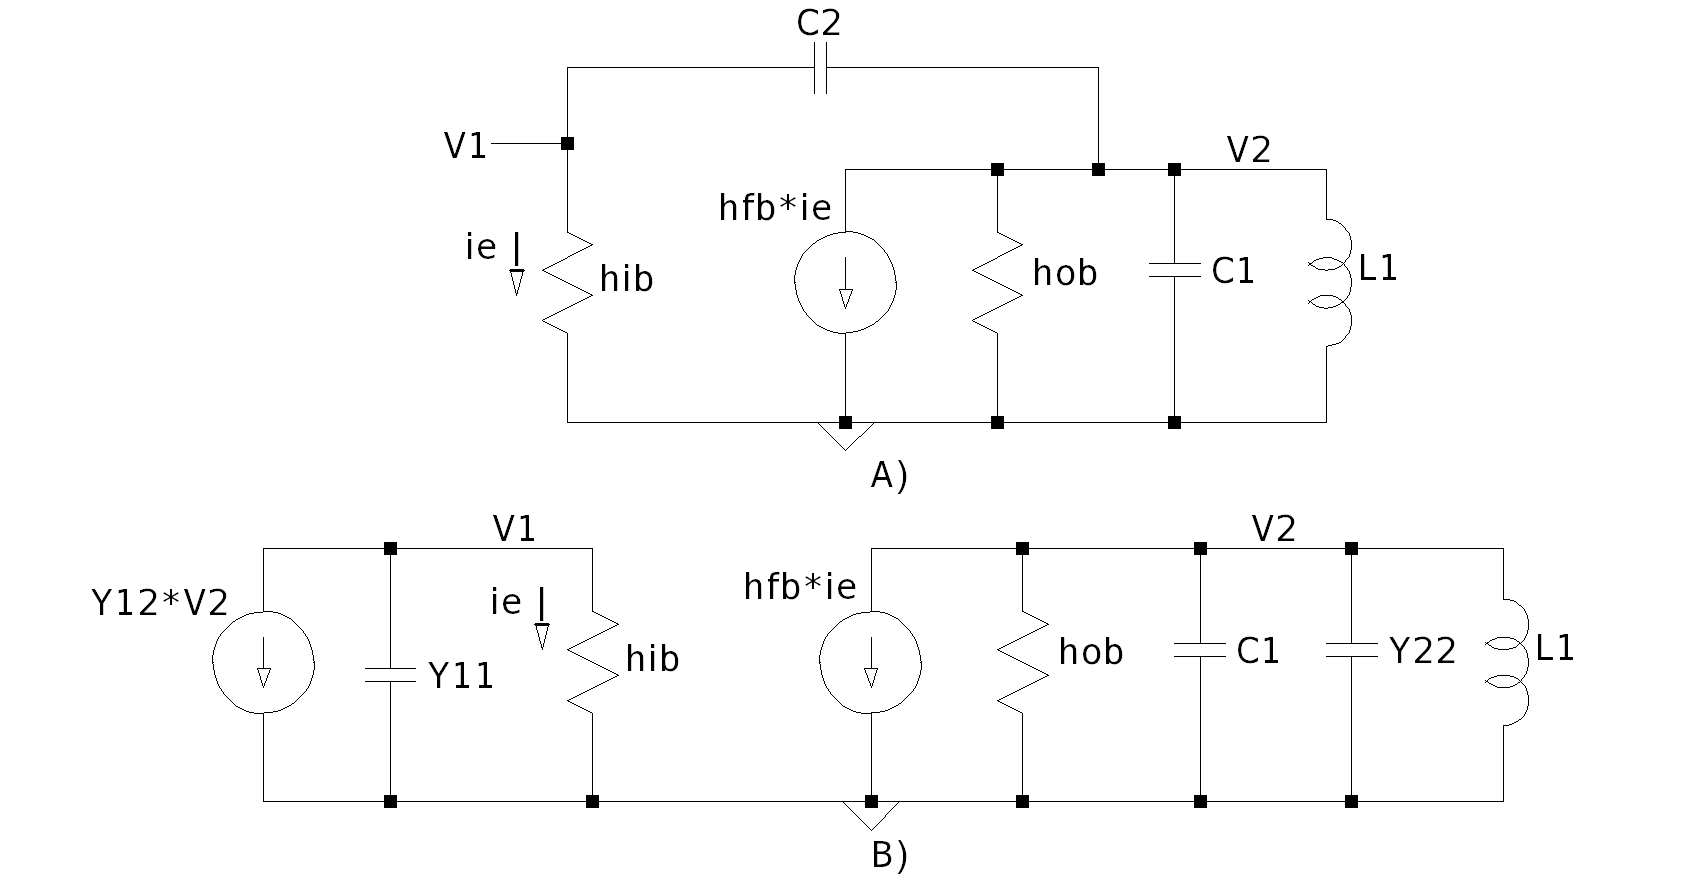
\includegraphics[scale=1, width=.8\textwidth]{small_signal_tx}
    \caption{A) Modelo en pequeña señal del bucle de oscilación para frecuencias medias B) Modelo en pequeña señal del oscilador sustituyendo el condensador de realimentación $C_1$ por su equivalente en parámetros $Y$}
    \label{fig:ss_tx}
\end{figure}

\paragraph{Modelo en pequeña señal:} ANADIR LOS CALCULOS DE LA INDUCTANCIA APROX 200N SEGUN INTERESE. El objetivo de este modelo es el cálculo de la frecuencia de resonancia del oscilador. En la figura \ref{fig:ss_tx} se muestra el modelo en pequeña señal del oscilador para frecuencias intermedias, entorno a la frecuencia de oscilaci\'on. El bucle de oscilaci\'on se trata de una realimentación paralelo-paralelo, por lo que se representa el condensador de realimentación $C_1$ como su equivalente en par\'ametros $Y$. El valor de dichos par\'ametros son:
\[
\begin{array}{rl} 
      \begin{array}{l}
	 Y_{11} = \frac{i_1}{v_1}|_{v_2 = 0} = s \cdot C_2 \\
	 Y_{12} = \frac{i_1}{v_2}|_{v_1 = 0} = -s \cdot C_2 
      \end{array}
      &
      \begin{array}{l}
	 Y_{21} = \frac{i_2}{v_1}|_{v_2 = 0} = -s \cdot C_2 \\
	 Y_{22} = \frac{i_2}{v_2}|_{v_1 = 0} = s \cdot C_2 
      \end{array}
\end{array}
\]
\paragraph{}
Se deben tener en cuenta ciertas consideraciones previas como consecuencia del an\'alisis del esquema B) en la figura \ref{fig:ss_tx}. La realimentaci\'on es positiva en el momento que $Y_{12}<0$ y $h_{fb}<0$ por lo que $V_2>0$. El modelo que se muestra corresponde a frecuencias intermedias entorno a la de oscilaci\'on. Para frecuencias bajas, la impedancia de $C_2$ tendrá un valor tan alto que corta la realimentación ,siguiendo el esquema A) figura \ref{fig:ss_tx}. para frecuencias altas, la impedancia de $C_2$ tendr\'a un valor tan bajo que supondr\'a un cortocircuito a tierra para la corriente de realimentaci\'on, por lo que $ie = 0 \unit{\ampere}$.
\paragraph{}
Se calcula la frecuencia de resonancia, en base al modelo B) de la figura \ref{fig:ss_tx}. Siguiendo el criterio de Barkhausen la frecuencia de resonancia se corresponde con la única con desfase $\angle A_l(f_0) = \SI{180}{\degree}$ a lo largo del bucle y una magnitud $|A_l(f_0)|\ge 0$. Se obtiene la funci\'on de transferencia de la ganancia en lazo abierto.
Siguiendo el modelo general de la realimentaci\'on ecuaci\'on \ref{eq:feedback} aplicada al esquema B) de la figura \ref{fig:ss_tx}, se calcula: 
\begin{equation}
f = Y_{12} = -s \cdot C1 
\end{equation}
\paragraph{}
Se muestra el desarrollo para el c\'alculo de $A = \frac{V_2}{i_E}$:
\[
\begin{array}{rl} 
      \begin{array}{l}
   \frac{i_E}{V_1} = Y_{T1} = s\cdot C_2 + \frac{1}{h_{ib}} \\
   \frac{i_e}{V_{1}} = \frac{1}{h_{ib}} \\
   i_E = Y_{T1} \cdot i_e \cdot h_{ib}
      \end{array}
      &
      \begin{array}{r}
   \frac{V_2}{h_{fb}\cdot i_e} = {Y_{T2}}^{-1} \\
   Y_{T2} = s\cdot C_2 + s\cdot C_1 + \frac{1}{s\cdot L_1} + h_{ob} \\
   V_2 = \frac{h_{fb}\cdot i_e}{Y_{T2}} 
      \end{array}
\end{array}
\]
\begin{equation}
   A = \frac{-h_{fb}}{Y_{T1} \cdot Y_{T2} \cdot h_{ib}} 
\end{equation}
\paragraph{}
Se calcula la ganancia en lazo abierto como $A_l = A \cdot f$ y sustituyendo los valores de $Y_{T1}$ e $Y_{T2}$:
\begin{equation}
   \label{eq:Al_tx}
   A_l = \frac{h_{fb} \cdot C_1 \cdot s^2}{ \left( C_2+C_1 \right) \left( s \cdot h_{ib} \cdot C_2 + 1\right) \left( s^2 + s \cdot \frac{h_{ob}}{C_1 + C_2} + \frac{1}{(C_1 + C_2)\cdot L_1}\right) }
\end{equation}
\paragraph{}
Al observar la expresi\'on obtenida en la ecuaci\'on \ref{eq:Al_tx}, se sacan conclusiones para esbozar el diagrama de Bode de manera anal\'itica. En primer lugar, se analiza el desfase, el cual a bajas frecuencias es 0, debido a la suma de los \SI{180}{\degree} del cero doble junto a los \SI{180}{\degree} de $h_{fb}$. El polo cuadr\'atico introduce un desfase de \SI{-180}{\degree}, al que se llega de manera asint\'otica pero de forma r\'apida debido al bajo valor del coeficiente de amortiguaci\'on. Si a este hecho se le añaden los \SI{-90}{\degree} del polo simple, se obtiene que la frecuencia de resonancia con desfase \SI{180}{\degree} se encontrará en algún lugar entre el polo simple y el polo cuadrático.
\paragraph{}
Se esboza el diagrama de bode para los valores obtenidos en el apartado de polarizaci\'on (ecuaciones \ref{eq:result_pol1} y \ref{eq:result_pol2}) junto a los siguientes valores de los elementos 
$$ L_1 = \SI{630}{\nano\henry} \quad C_1=\SI{47}{\pico\farad} \quad C_2=\SI{47}{\pico\farad} $$
\begin{figure}[h]
    \centering
    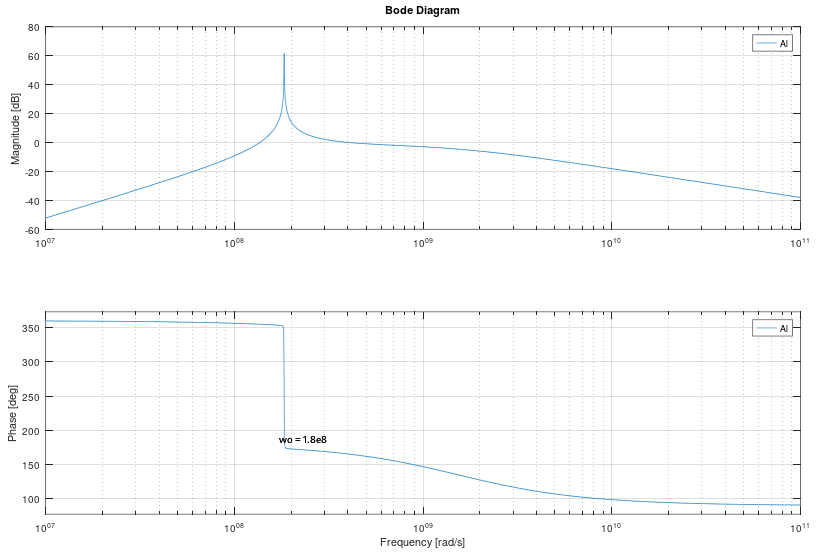
\includegraphics[scale=1, width=.8\textwidth]{bode_tx}
    \caption{Diagrama de Bode de la ganancia en lazo abierto del oscilador $A_l$ para frecuencias intermedias}
    \label{fig:bode_tx}
\end{figure}
En el diagrama de Bode de la figura \ref{fig:bode_tx}, se obtiene una frecuencia angular $\omega_0 = \SI{1.8e8}{\radian\per\second}$, por lo que se obtiene una frecuencia de resonancia de:
\begin{equation}
   f_0 = \frac{\omega_0}{2\cdot\pi} = \SI{28.65}{\mega\hertz}
\end{equation}
\paragraph{}
La obtenci\'on del diagrama de Bode se ha conseguido por medio del programa de c\'alculo computacional Octave REFERENCIA

\paragraph{} la señal digital de inicio o corte es producida por el microcontrolador Atmega328p, y se desarrollará en el correspondiente apartado CITAR. El transistor PNP es utilizado como conmutador.

\paragraph{Antena} CALCULOS DEL TRANSFORMADOR, EXPLICAR EL CONDENSADOR ES PARA QUE AL TOCARLA NO PASE NADA.
simulacion de potencia disipada por la antena?
\paragraph{Resultado de la Simulaci\'on} SIMULACION LTSPICE
son 3 capturas una la de la oscilacion con las medidas de frecuencia.
una general con varios ciclos de digitalin.
otra del flanco de subida y bajada de digitalin con vout y vbe viendo como se corta el transistor.
\paragraph{Resultado de la pr\'actica} CAPTURA DEL OSCILOSCOPIO Y MEDIDA DE CORRIENTE
\paragraph{}
Explicacion de la relevancia de una buena antena en transmision, el cuerpo humano como antena(bibliografia)

% \paragraph{Modulaci\'on de los canales mediante NE555}
% \paragraph{}
% La estrategia para la modulaci\'on reside en concepto de NE555 es un chip, el cual, configurado adecuadamente puede trabajar como un astable. Adem\'as, la frecuencia de oscilación del astable puede ser variada en función de los elementos de configuración. La idea es utilizar la señal proporcionada por el chip para cortar el oscilador según la frecuencia del NE555, realizando una mezcla de ambas señales y dando lugar a la señal modulada ASK. La mezcla se realiza por medio del transistor Q2 PNP, el cual trabaja en corte y saturación.
% \paragraph{}
% La configuraci\'on de astable para el chip NE555 viene dada en la datasheet del mismo, por lo que se sigue el modelo de esta configuraci\'on. El chip soporta un rango de tensiones de alimentaci\'on $4.5 < V_{CC} < 16$ \unit{\volt}, por lo que se ajusta a las condiciones del trabajo. Se realiza el diseño y el valor de los componentes siguiendo las siguientes ecuaciones proporcionadas por la hoja de datos:
% 
% \begin{align} 
%    \label{eq:freq}
%    Freq &= \frac{1.44}{(R_A + 2 \cdot R_B) \cdot C} \\
%    \label{eq:duty}
%    Duty &= \frac{1.44}{(R_A + 2 \cdot R_B)}
% \end{align}
% 
% Se requiere un ciclo de trabajo de aproximadamente $Duty \approx 0.5$ por lo que $R_B >> R_A$. La frecuencias de la onda cuadrada moduladora son de \SI{15}{\kilo\hertz} y \SI{3}{\kilo\hertz} para distintos valores de $R_B$. Estas frecuencias son alternadas mediante dos pulsadores los cuales conectan los dos distintos valores de $R_B$ al circuito tras ser accionados, generando as\'i dos distintos canales digitales. Cabe mencionar que $R_A$ no puede ser arbitrariamente pequeña, pues el el esquema eléctrico del chip que proporciona el fabricante, $R_A$ se conecta como resistencia de colector del transistor de \textit{DISCH}. Hacer $R_A$ más pequeño incurre en mayor consumo del chip en cada semiciclo.
% \paragraph{}
% Las frecuencias de modulación se eligen teniendo en cuenta: la facilidad de filtrado con respecto a las bajas frecuencias, los valores de $R_B$ y $R_A$, y la frecuencia de muestreo del ADC en el decodificador digital. Teniendo en cuenta estos parámetros, se calculan $R_A$ y $R_B$ con las ecuaciones.
% \paragraph{}
% En primer lugar, se selecciona $R_A$ para obtener un consumo razonable de descarga siguiendo la ecuaci\'on $I_{Disch} = \frac{V_{CC}-0.2}{R_A}$, un valor de $R_A = \SI{500}{\ohm}$ da lugar a $I_{Disch} = \SI{17.6}{\milli\ampere}$, lo cual es aceptable. En segundo lugar se debe fijar el ciclo de trabajo, si se hace $R_B = 10 \cdot R_A$ es una aproximaci\'on suficiente, ya que, mediante la ecuaci\'on \ref{eq:duty} queda $Duty = 0.476 \approx 0.5$. Por \'ultimo se fijan las frecuencias de modulaci\'on mediante la ecuaci\'on \ref{eq:freq}, lo cual nos fija un valor de $C$. Al tener dos diferentes canales con dos valores de frecuencia y $R_B$, se obtiene el siguiente sistema de ecuaciones para obtener el valor de $C$:
% \begin{align*} 
%    Freq_1 &= \frac{1.44}{(R_A + 2 \cdot R_{B1}) \cdot C} \\
%    Freq_2 &= \frac{1.44}{(R_A + 2 \cdot R_{B2}) \cdot C} \\
% \end{align*}
% 
% siendo  $Freq_1= \SI{15}{\kilo\hertz}$ $Freq_2=\SI{3}{\kilo\hertz}$ $R_{B1}=\SI{10}{\kilo\ohm}$ $R_{B2}=\SI{5}{\kilo\ohm}$, el valor de $C$ como resultado es $C \approx \SI{6.8}{\nano\farad}$



